% *********************************************************
% Check "thesis-style.sty" to customise language and others
% *********************************************************

\documentclass[a4paper,12pt,twoside]{ThesisStyle}
\usepackage{thesis-style}

\newcommand{\titlemark}{Desenvolupament d’una aplicació òbil de codi obert per a fer pagaments entre usuaris mitjaçant codis QR} % Project title for custom header
\newcommand{\documentmark}{Memòria} % Document type for custom header
\newcommand{\appendixmark}{Annex} % Appendix mark for custom header

% \cftsetindents{section}{1em}{3em}
% \setlength\cftsectionnumwidth{4em} % uncomment to see difference

\begin{document}

\frontmatter

\pagenumbering{gobble}

\thispagestyle{empty}
\begin{table}[htb]
\centering
\begin{Large}
\resizebox{\textwidth}{!}{\begin{tabular}{ | l |}
 \hline
 \\

\includegraphics[scale=0.9]{imatges/logo_eps.png} \\[0.7cm]
\centerline{Projecte fi de grau}\\[1cm]
\hline
\\
Estudi: Grau en Enginyeria Informàtica\\[0.7cm]
\hline
\\
Títol: Desenvolupament d'una aplicació mòbil de codi obert per a fer pagaments\\
entre usuaris mitjaçant codis QR\\[0.7cm]
\hline
\\
Document: Memòria\\[0.7cm]
\hline
\\
Alumne: Sudan Wu\\[0.7cm]
\hline
\\
Tutor: Pau Xiberta i Armengol\\
Departament: INFORMÀTICA, MATEMÀTICA APLICADA I ESTADÍSTICA\\
Àrea: LLENGUATGES I SISTEMES INFORMÀTICS\\[0.7cm]
\hline
\\
Convocatòria (Setembre/2024): XXX\\[0.7cm]
\hline

\end{tabular}}
\end{Large}
\end{table}

\newpage

\begin{titlepage}

% Upper part of the page

\includegraphics[scale=0.9]{imatges/logo_eps.png} \\[1cm]
\begin{center}
\textsc{\Large Projecte Fi de Grau} \\[1cm]

% Title
\begin{spacing}{2}
\HRule \\
\textbf{\Huge Títol del projecte} \\
\HRule \\[0.5cm]
\end{spacing}

% Author and supervisor and other data
{
\large
\emph{Autor:} \\
Nom \textsc{Sudan Wu} \\[1cm]
Setembre 2024 \\[1cm]
Grau en Enginyeria Informàtica \\[1cm]
\emph{Tutor:} \\
Nom \textsc{Pau Xiberta i Armengol} \\
}

\end{center}
\end{titlepage}

\titlepage

\dominitoc

\pagenumbering{roman}

\chapter*{Resum}
\label{chp:resum}



\chapter*{Agraïments}
\label{chp:agraiments}

Per començar vull agrair molt especialment a al meu tutor Pau Xiberta i Armengol, per la seva guia, paciència i saviesa durant tot el procés. Les seves orientacions han estat fonamentals per a la consecució d’aquest treball, i la seva dedicació ha estat una font constant de motivació.\\

També voldria agrair als meus companys i amics per estar sempre al meu costat, oferint suport emocional i consells valuosos en moments de dubte i incertesa. La vostra companyia ha fet aquest viatge molt més suportable i enriquidor.\\

No puc oblidar la meva família, que ha estat el meu pilar més ferm al llarg de tota aquesta etapa acadèmica. Gràcies per creure en mi, per la vostra paciència infinita i per animar-me a seguir endavant, fins i tot en els moments més difícils.\\

Finalment, vull reconèixer l’esforç i dedicació de tots els professors que m’han format durant aquests anys. Les vostres ensenyances han estat fonamentals per arribar fins aquí, i cada una de les vostres lliçons ha deixat una petjada en aquest treball.\\

A tots, gràcies de tot cor per fer possible aquest assoliment.


\tableofcontents

\listoffigures

\listoftables

\mainmatter



\chapter{Introducció, motivació, finalitat i objectius del projecte}
\label{chp:intro}

\section{Introducció}
\label{sec:introduccio}

A l'hora de processar un pagament, la majoria de botigues utilitzen un Terminal Punt de Venda (TPV) físic, i els clients fan servir una targeta bancària o una cartera digital que incorpora aquesta targeta. El TPV actua com a intermediari en l'operació, introduint un procés addicional que pot augmentar tant els costos com el risc d'errors. Tot i que existeixen plataformes de pagament en línia, aquestes no estan dissenyades per substituir completament el TPV físic, i sovint no són de codi obert ni ofereixen l'opció de realitzar transaccions mitjançant codis QR.

\section{Motivació}
\label{subsec:motivacio}

L’evolució tecnològica i la digitalització han transformat profundament la manera com les empreses gestionen els seus processos de pagament. Tot i els avenços, el sistema tradicional basat en terminals físics de punt de venda (TPV) encara predomina, arrossegant amb si costos operatius elevats i riscos associats a errors humans i fraus. Aquesta situació, sumada a la creixent adopció de tecnologies de pagament mòbil i l’ús de codis QR en diverses parts del món, posa de manifest la necessitat d’explorar alternatives més eficients, segures i accessibles.

Aquest projecte neix de la voluntat d’abordar aquestes limitacions, oferint una solució que pugui substituir o complementar els TPV físics amb una plataforma de pagament en línia de codi obert. Una solució que permeti als comerciants processar transaccions mitjançant codis QR, oferint així una experiència de pagament més ràpida, senzilla i segura tant per a les botigues com per als clients.

La motivació principal d’aquest projecte és reduir els costos operatius i minimitzar els riscos associats als sistemes de pagament tradicionals, alhora que es promou la inclusió tecnològica a través d’una eina de codi obert, accessible per a qualsevol empresa o desenvolupador que desitgi implementar-la. Creiem que, mitjançant aquesta iniciativa, podem contribuir a la transformació digital del comerç, afavorint la seva competitivitat i adaptabilitat en un mercat cada cop més globalitzat i dinàmic.

\section{Objectius}
\label{subsubsec:objectius}

L'objectiu d'aquest treball de final de grau és desenvolupar una aplicació full stack que inclogui totes les funcions necessàries per gestionar pagaments mitjançant codis QR. Aquest desenvolupament inclourà:

\begin{itemize}
  \item El disseny i la implementació de la base de dades per emmagatzemar la informació de les transaccions i els usuaris.
  \item El desenvolupament d'una API que permeti interactuar de manera eficient amb la base de dades, facilitant la creació, gestió i consulta de pagaments.
  \item La creació d'una interfície d'usuari senzilla i intuïtiva, que permeti als usuaris generar i escanejar codis QR per realitzar transaccions.
  \item El desenvolupament de les aplicacions frontals basades en web que permetin als usuaris accedir al sistema, generar codis QR i realitzar els pagaments de manera segura i ràpida.
\end{itemize}

L'aplicació permetrà als comerciants generar codis QR per a cada transacció, que els clients podran escanejar amb el seu dispositiu mòbil per efectuar el pagament.

A més, com a funcionalitats futures, tot i que no són prioritàries en aquesta fase inicial del projecte, el sistema també podria incloure:

\begin{itemize}
  \item Una pàgina d'anàlisi que proporcioni informació detallada sobre les transaccions realitzades, ajudant els comerciants a gestionar millor les seves vendes.
  \item Un sistema de subscripcions que permeti als clients realitzar pagaments recurrents de manera automàtica.
\end{itemize}

Aquestes funcionalitats addicionals estan pensades per ampliar les capacitats del sistema i oferir un valor afegit tant als comerciants com als clients, contribuint així a una experiència de pagament més fluida i moderna.



\chapter{Viabilitats}
\label{chp:viabilitats}

\section{Viabilitat tècnica}
\label{subsec:Viabilitat tècnica}

L'aplicació utilitzarà Node.js (apollo server) per a la gestió del servidor i flutter per al desenvolupament de la interfície d'usuari. A més, es farà servir una base de dades en MongoBD per emmagatzemar les transaccions i informació dels usuaris. Aquestes tecnologies són àmpliament utilitzades i ben suportades per la comunitat de desenvolupadors.

La infraestructura es basarà en serveis en núvol per garantir la disponibilitat i escalabilitat de l'aplicació. Els costos associats amb l'allotjament en el núvol seran monitoritzats per assegurar l'eficiència econòmica.

\section{Viabilitat econòmica}
\label{subsec:Viabilitat económica}

Els costos principals del projecte inclouen el desenvolupament de l'aplicació, que es realitzarà internament, i els costos d'allotjament en el núvol, que seran proporcionats per serveis com AWS amb un pressupost de X euros mensuals.

El sistema de pagament mitjançant codis QR ofereix una solució econòmica en comparació amb els terminals de TPV tradicionals, amb una possible font d'ingressos a través de comissions per transacció i opcions de subscripció per serveis addicionals.


\section{Viabilitat temporal}
\label{subsec:Viabilitat temporal}

El projecte es completarà en X mesos, amb un pla detallat que cobreix les fases de disseny, desenvolupament, proves i desplegament. La fase de proves serà especialment important per garantir la seguretat i l'eficiència del sistema.

Un possible risc és la integració amb els sistemes de pagament de tercers, que podria requerir més temps del previst si es presenten problemes de compatibilitat.


\section{Viabilitat de mercat}
\label{subsec:Viabilitat de mercat}

Amb l'augment de l'ús de pagaments mòbils i la necessitat de solucions de pagament contactless, hi ha una demanda creixent per a sistemes de pagament basats en codis QR. Aquesta tendència proporciona una oportunitat significativa per a la nostra aplicació.

Encara que hi ha altres solucions de pagament basades en codis QR, el nostre sistema es diferencia per la seva integració fàcil amb altres plataformes i la seva estructura de codi obert, que permet personalització i adaptació a les necessitats específiques dels usuaris.

\section{Viabilitat Legal i Ètica}
\label{subsec:Viabilitat Legal i Ètica}

L'aplicació serà dissenyada per complir amb les regulacions de protecció de dades com el GDPR (General Data Protection Regulation), garantint que la informació dels usuaris es gestioni de manera segura i conforme a la legislació vigent.


\chapter{Metodologia}
\label{chp:metodologia}


\section*{Introduction}
\label{subsec: Introduction}

Per al desenvolupament de l'aplicació, es va utilitzar la metodologia àgil Scrum, tot i que es tractava d'un projecte individual. Scrum és conegut per la seva flexibilitat i per permetre gestionar projectes complexos a través de cicles iteratius de treball anomenats sprints. Encara que tradicionalment Scrum està dissenyat per a equips, es van adaptar els seus principis per optimitzar la gestió del temps i els recursos durant el desenvolupament del projecte.

L'elecció de Scrum es va basar en la necessitat de mantenir una alta capacitat de resposta davant els canvis en els requisits i per estructurar el procés de desenvolupament en fases manejables. Scrum va permetre dividir el projecte en sprints, cosa que va facilitar la planificació i el seguiment del progrés, assegurant-se que cada fase del projecte es completava abans de passar a la següent.

Per a la planificació del projecte, es van definir sprints de dues setmanes, cadascun amb objectius específics que havien de complir-se abans de començar el següent sprint. Al principi de cada sprint, es va elaborar un pla detallat de les tasques a realitzar, prioritzant les més crítiques i assegurant-se que estaven alineades amb els objectius generals del projecte.

Durant cada sprint, es va utilitzar una adaptació de les reunions diàries (normalment utilitzades en equips) per reflexionar diàriament sobre el progrés i identificar possibles impediments. Aquest procés va ajudar a mantenir el focus i ajustar els plans si era necessari.

Es va crear i gestionar un product backlog on es llistaven totes les funcionalitats a desenvolupar. Aquest backlog es va prioritzar d’acord amb la seva importància i la complexitat de la implementació. Cada sprint es va planificar tenint en compte aquesta llista, assegurant-se que sempre es treballava en les tasques més rellevants per al progrés del projecte.

L'ús de Scrum, adaptat a un entorn individual, va ser fonamental per a la gestió eficient del temps i la consecució dels objectius del projecte. Va permetre que el desenvolupament es realitzés de manera ordenada i progressiva, proporcionant la flexibilitat necessària per fer ajustos sobre la marxa. Aquesta metodologia va resultar especialment útil per mantenir el ritme de treball i assegurar que cada fase del projecte es completés amb èxit abans de passar a la següent.

\section{Gestió de projecte}
\label{subsec: Gestió de projecte}


\textbf{Pasos per a Scrum Personal}
\begin{itemize}
    \item \textbf{Propietari del producte: }En aquest context, tu mateix ets el Product Owner. Ets responsable de definir els teus objectius personals, prioritzar les teves tasques i assegurar-te que estàs treballant en el més important en tot moment.
    \item \textbf{Iteracions: }Defineix períodes de temps, anomenats Iteracions o Sprints, durant els quals t'enfocaràs a completar una sèrie de tasques. Aquests sprints poden ser d'una setmana, dues setmanes o qualsevol altra durada que et resulti efectiva.
    \item \textbf{Llista de Tasques: }Crea una llista de tasques pendents que necessites realitzar. Aquestes tasques poden ser objectius a llarg termini, projectes més grans desglossats en tasques més petites o simplement activitats quotidianes.
    \item \textbf{Planificació del Sprint Personal: }Al començament de cada Sprint, selecciona les tasques que vols completar durant aquell període. Prioritza-les segons la seva importància i estableix objectius assolibles per al Sprint.
    \item \textbf{Reunions Diàries: }Reserva uns minuts cada dia per reflexionar sobre el teu progrés. Què vas fer ahir? Què planeges fer avui? Hi ha algun obstacle que estigui impedint el teu progrés?
    \item \textbf{Revisió del Sprint Personal: }Al final de cada Sprint, revisa el que has aconseguit i avalua el teu progrés cap als teus objectius. Has completat totes les tasques que t'havies proposat? Què tan efectiu va ser el teu pla? Què pots millorar per al pròxim Sprint?
    \item \textbf{Retrobament Personal: }Dedica temps al final de cada Sprint per reflexionar sobre el teu procés de treball. Identifica què va funcionar bé, què no va funcionar tan bé i quins canvis pots realitzar per millorar la teva productivitat i eficiència en el pròxim Sprint.
\end{itemize}


\begin{figure}[h] % [h] indica que vols col·locar la figura aquí mateix
  \centering
  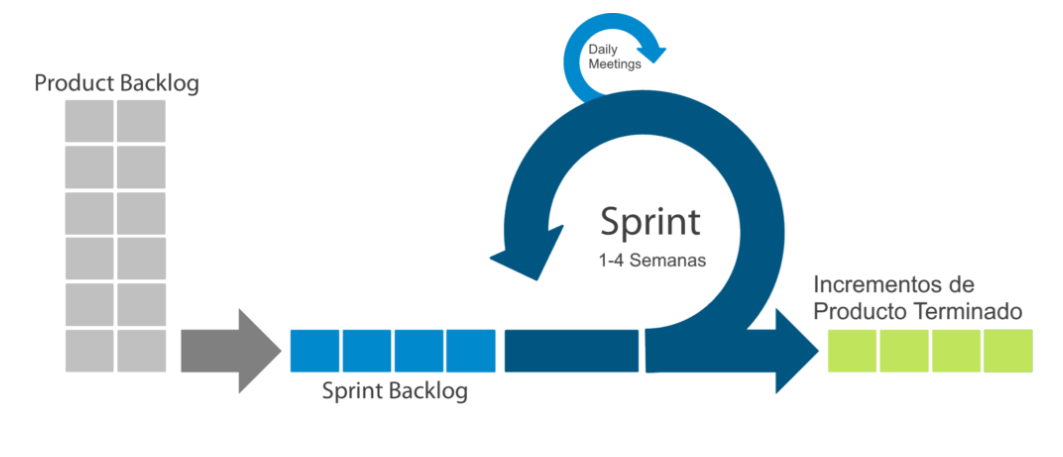
\includegraphics[width=\linewidth]{imatges/scrum.png} % ajusta l'amplada si cal
  \caption{Aquest és el títol de la figura.}
  \label{fig:exemple_figura}
\end{figure}




\chapter{Planificació}
\label{chp:planificació}





\chapter{Marc de treball i conceptes previ}
\label{chp:marcdetreball}



\chapter{Requisits del sistema}
\label{chp:requisits}



\chapter{Estudi i decisions}
\label{chp:estudi}



\chapter{Anàlisi i disseny del sistema}
\label{chp:analisi}



\chapter{Implementació i proves}
\label{chp:implementacio}



\chapter{Implantació i resultats}
\label{chp:implantacio}

\section{Prova 1}
\section{Prova 2}
\section{Prova 3}
\section{Prova 4}
\section{Prova 5}
\section{Prova 6}
\section{Prova 7}
\section{Prova 8}
\section{Prova 9}
\section{Prova 10}
\section{Prova 11}



\chapter{Conclusions}
\label{chp:conclusions}



\chapter{Treball futur}
\label{chp:treballfutur}



% \backmatter % From this point, chapters are unnumbered


%%%%%%%%%%%%%%%%%%%%%%%%%%%%%%%%%%%%%%%%%%%%
% GETI projects: bibliography as a chapter
%%%%%%%%%%%%%%%%%%%%%%%%%%%%%%%%%%%%%%%%%%%%
%\chapter{Bibliografia}
%\renewcommand{\bibsection}{} % Remove intrinsic bibliography name

\bibliographystyle{ThesisStyleBreakable}
\bibliography{bibliography}

%%%%%%%%%%%%%%%%%%%%%%%%%%%%%%%%%%%%%%%%%%%%
% GETI projects: move "\backmatter" after bibliography to allow unnumbered appendices
%%%%%%%%%%%%%%%%%%%%%%%%%%%%%%%%%%%%%%%%%%%%
% \backmatter



% APPENDICES

% 1. Short and limited command for appendices:
% \appendix

% 2. Full command for appendices (package 'appendices' needed in the preamble: check 'thesis-style.sty'):
% \usepackage[title]{appendix} % add 'titletoc' to add "Appendix" to ToC

% \begin{appendices}

% To manually set appendix chapter names (should be after "\backmatter"):
% \renewcommand{\chaptermark}[1]{\markboth{#1}{}}
% \chapter{Appendix A. Appendix name}

% To let the package manage appendix chapter names (before "\backmatter"):
% \chapter{Appendix name}

% Alternative for separated appendices:
% \include{Appendix1}

% \end{appendices}

% 3. No command for appendices (just unnumbered chapters):
% \renewcommand{\chaptermark}[1]{\markboth{#1}{}}
% \chapter{Appendix A. Appendix name}


%%%%%%%%%%%%%%%%%%%%%%%%%%%%%%%%%%%%%%%%%%%%
% GETI projects: change header to show appendix mark
%%%%%%%%%%%%%%%%%%%%%%%%%%%%%%%%%%%%%%%%%%%%
% \fancyhead[RE,LO]{\bfseries\color{black}\appendixmark}    % Appendix mark (boldface) in the right on even pages, and in the left on odd pages


\renewcommand\appendixname{Annex} % Appendix name (change default)

\begin{appendices}

\chapter{Pressupost}

Lorem ipsum dolor sit amet, consectetur adipiscing elit. Nunc congue mattis tellus, in rhoncus nisl laoreet vel. Sed nulla libero, tincidunt id ligula congue, hendrerit maximus mi. Morbi nec metus in urna imperdiet mattis pretium a libero. Fusce est mauris, convallis id facilisis faucibus, consequat aliquet eros. Vivamus et dui pulvinar, rutrum velit at, volutpat tellus. Nulla vehicula ullamcorper justo, blandit interdum leo sagittis quis. Quisque convallis vel ante ac rutrum. Morbi et varius sem, sed tristique elit. Vestibulum aliquam facilisis pellentesque. Suspendisse consequat commodo eros, sit amet tincidunt sapien semper in. Nunc ut magna ac quam tempor malesuada et at ex. Donec mattis mauris ante, id condimentum elit dapibus at.

Curabitur ut sodales sapien. Etiam eget ultrices risus, in dignissim nunc. Quisque quis tortor in nunc posuere lacinia ut sed dui. Praesent ut sollicitudin diam, ut mattis magna. Morbi porttitor fermentum magna a pharetra. Nullam at magna diam. Suspendisse vehicula tellus eget ligula aliquam semper. Integer sed ullamcorper felis, ac imperdiet elit. Praesent eu suscipit ligula, sit amet vulputate erat. Etiam eget tempor est, vitae aliquet tortor. Nam efficitur tristique ligula. Aliquam blandit leo non ante suscipit, vitae mattis diam rhoncus. Ut ac dui sit amet dui venenatis suscipit.

Nunc sollicitudin hendrerit risus, quis ultricies orci elementum non. Aliquam erat volutpat. Mauris neque turpis, molestie in tellus id, pharetra gravida mi. Suspendisse potenti. Donec aliquam dolor eu pellentesque auctor. Proin eget sapien ut tellus maximus lacinia. Praesent blandit pretium mi, suscipit sollicitudin eros iaculis in. Nunc a justo sit amet mauris auctor posuere sit amet vel erat. Etiam in maximus nisi. Pellentesque blandit pharetra lectus nec efficitur. Praesent tristique vel arcu id bibendum. In eget eros fringilla magna hendrerit facilisis ac vitae urna. Donec malesuada fermentum dictum. Pellentesque aliquet tortor vitae suscipit tempus. Phasellus ornare risus mi, vel placerat justo efficitur eu. Phasellus quis tincidunt enim.

Etiam a elementum lorem. Integer ac lectus hendrerit, venenatis ante vitae, accumsan eros. Orci varius natoque penatibus et magnis dis parturient montes, nascetur ridiculus mus. Curabitur non varius dolor. Donec suscipit metus vitae ultrices sagittis. Praesent ac dapibus justo, vel mollis sapien. Pellentesque at iaculis neque. Donec ac tellus orci. Pellentesque eleifend fringilla massa, in lobortis nibh finibus in. Morbi ut neque vitae est congue tempor efficitur imperdiet dolor. Pellentesque nec nibh nec nibh fringilla laoreet. Duis fermentum ornare sollicitudin. Maecenas finibus tincidunt justo commodo commodo. Suspendisse venenatis odio dignissim auctor elementum. Duis non mauris orci.

Lorem ipsum dolor sit amet, consectetur adipiscing elit. Nunc congue mattis tellus, in rhoncus nisl laoreet vel. Sed nulla libero, tincidunt id ligula congue, hendrerit maximus mi. Morbi nec metus in urna imperdiet mattis pretium a libero. Fusce est mauris, convallis id facilisis faucibus, consequat aliquet eros. Vivamus et dui pulvinar, rutrum velit at, volutpat tellus. Nulla vehicula ullamcorper justo, blandit interdum leo sagittis quis. Quisque convallis vel ante ac rutrum. Morbi et varius sem, sed tristique elit. Vestibulum aliquam facilisis pellentesque. Suspendisse consequat commodo eros, sit amet tincidunt sapien semper in. Nunc ut magna ac quam tempor malesuada et at ex. Donec mattis mauris ante, id condimentum elit dapibus at.

Curabitur ut sodales sapien. Etiam eget ultrices risus, in dignissim nunc. Quisque quis tortor in nunc posuere lacinia ut sed dui. Praesent ut sollicitudin diam, ut mattis magna. Morbi porttitor fermentum magna a pharetra. Nullam at magna diam. Suspendisse vehicula tellus eget ligula aliquam semper. Integer sed ullamcorper felis, ac imperdiet elit. Praesent eu suscipit ligula, sit amet vulputate erat. Etiam eget tempor est, vitae aliquet tortor. Nam efficitur tristique ligula. Aliquam blandit leo non ante suscipit, vitae mattis diam rhoncus. Ut ac dui sit amet dui venenatis suscipit.

Nunc sollicitudin hendrerit risus, quis ultricies orci elementum non. Aliquam erat volutpat. Mauris neque turpis, molestie in tellus id, pharetra gravida mi. Suspendisse potenti. Donec aliquam dolor eu pellentesque auctor. Proin eget sapien ut tellus maximus lacinia. Praesent blandit pretium mi, suscipit sollicitudin eros iaculis in. Nunc a justo sit amet mauris auctor posuere sit amet vel erat. Etiam in maximus nisi. Pellentesque blandit pharetra lectus nec efficitur. Praesent tristique vel arcu id bibendum. In eget eros fringilla magna hendrerit facilisis ac vitae urna. Donec malesuada fermentum dictum. Pellentesque aliquet tortor vitae suscipit tempus. Phasellus ornare risus mi, vel placerat justo efficitur eu. Phasellus quis tincidunt enim.

Etiam a elementum lorem. Integer ac lectus hendrerit, venenatis ante vitae, accumsan eros. Orci varius natoque penatibus et magnis dis parturient montes, nascetur ridiculus mus. Curabitur non varius dolor. Donec suscipit metus vitae ultrices sagittis. Praesent ac dapibus justo, vel mollis sapien. Pellentesque at iaculis neque. Donec ac tellus orci. Pellentesque eleifend fringilla massa, in lobortis nibh finibus in. Morbi ut neque vitae est congue tempor efficitur imperdiet dolor. Pellentesque nec nibh nec nibh fringilla laoreet. Duis fermentum ornare sollicitudin. Maecenas finibus tincidunt justo commodo commodo. Suspendisse venenatis odio dignissim auctor elementum. Duis non mauris orci.

Lorem ipsum dolor sit amet, consectetur adipiscing elit. Nunc congue mattis tellus, in rhoncus nisl laoreet vel. Sed nulla libero, tincidunt id ligula congue, hendrerit maximus mi. Morbi nec metus in urna imperdiet mattis pretium a libero. Fusce est mauris, convallis id facilisis faucibus, consequat aliquet eros. Vivamus et dui pulvinar, rutrum velit at, volutpat tellus. Nulla vehicula ullamcorper justo, blandit interdum leo sagittis quis. Quisque convallis vel ante ac rutrum. Morbi et varius sem, sed tristique elit. Vestibulum aliquam facilisis pellentesque. Suspendisse consequat commodo eros, sit amet tincidunt sapien semper in. Nunc ut magna ac quam tempor malesuada et at ex. Donec mattis mauris ante, id condimentum elit dapibus at.

Curabitur ut sodales sapien. Etiam eget ultrices risus, in dignissim nunc. Quisque quis tortor in nunc posuere lacinia ut sed dui. Praesent ut sollicitudin diam, ut mattis magna. Morbi porttitor fermentum magna a pharetra. Nullam at magna diam. Suspendisse vehicula tellus eget ligula aliquam semper. Integer sed ullamcorper felis, ac imperdiet elit. Praesent eu suscipit ligula, sit amet vulputate erat. Etiam eget tempor est, vitae aliquet tortor. Nam efficitur tristique ligula. Aliquam blandit leo non ante suscipit, vitae mattis diam rhoncus. Ut ac dui sit amet dui venenatis suscipit.

Nunc sollicitudin hendrerit risus, quis ultricies orci elementum non. Aliquam erat volutpat. Mauris neque turpis, molestie in tellus id, pharetra gravida mi. Suspendisse potenti. Donec aliquam dolor eu pellentesque auctor. Proin eget sapien ut tellus maximus lacinia. Praesent blandit pretium mi, suscipit sollicitudin eros iaculis in. Nunc a justo sit amet mauris auctor posuere sit amet vel erat. Etiam in maximus nisi. Pellentesque blandit pharetra lectus nec efficitur. Praesent tristique vel arcu id bibendum. In eget eros fringilla magna hendrerit facilisis ac vitae urna. Donec malesuada fermentum dictum. Pellentesque aliquet tortor vitae suscipit tempus. Phasellus ornare risus mi, vel placerat justo efficitur eu. Phasellus quis tincidunt enim.

Etiam a elementum lorem. Integer ac lectus hendrerit, venenatis ante vitae, accumsan eros. Orci varius natoque penatibus et magnis dis parturient montes, nascetur ridiculus mus. Curabitur non varius dolor. Donec suscipit metus vitae ultrices sagittis. Praesent ac dapibus justo, vel mollis sapien. Pellentesque at iaculis neque. Donec ac tellus orci. Pellentesque eleifend fringilla massa, in lobortis nibh finibus in. Morbi ut neque vitae est congue tempor efficitur imperdiet dolor. Pellentesque nec nibh nec nibh fringilla laoreet. Duis fermentum ornare sollicitudin. Maecenas finibus tincidunt justo commodo commodo. Suspendisse venenatis odio dignissim auctor elementum. Duis non mauris orci.

\chapter{Planificació}


\end{appendices}

% \printnomenclature

\end{document}
